\scanpage{93}
% manuscript lines 1–2
On suppose alors $V(f')$ et $V(f'')$ sont sans idéaux immergés

% manuscript lines 1–2
\margin{[il ne pourrait y en avoir qu'au pt $x$]}

% manuscript lines 3
[On peut $=$ les prendre intègres]

% manuscript lines 4–5
\[
\begin{aligned}
(V(f)\cap Z'_0={})\ V(f')\cap Z'_0&=\{x\}\\
(V(f)\cap Z''_0={})\ V(f'')\cap Z''_0&\unsure{\subseteq|=|\subset}\{x\}
\end{aligned}
\]

% manuscript lines 6–9
Il s'ensuit que $V(f)$ \uline{est sans} \uline{idéaux} immergés [et $=$ réduit si on veut], et que $V(f)$ est Coh. Mac. en dehors de $\{x\}$.

% manuscript lines 9
\figure{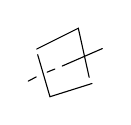
\begin{tikzpicture}[scale=.6,line cap=round]
\draw (.1,.95)--(.98,1.39)--(1.21,.35); \draw (.12,.83)--(.38,-.06)--(1.27,.22);
\draw (-.08,.27)--(.09,.36); \draw[dashed](.32,.46)--(.59,.57); \draw (.64,.59)--(1.49,.96);
\end{tikzpicture}}

% manuscript lines 9–13
\deleted{Donc au pt} Donc l'ens des pts où $X$ n'est pas Coh. Mac. est $Z=\deleted{\unsure{X}}Z'_0\cup Z''_0\cup D$, qui dans $X-V(f)$ est de codim $\leq\operatorname{codim}_{X'}Z'_0<n'\deleted{\unsure{1}}$, [car $Z'_0\ne\varnothing$, $Z'_0\ne\{x\}$], \deleted{et qui dans}

% manuscript lines 14–17
alors que la codim dans $V(f)$ de $V(f)\cap Z$ [i.e. l'ens des pts de $V(f)$ où \deleted{\unsure{Z}} il n'est pas Coh. Mac] est de codim $=\deleted{\unsure{\leq}}\dim V(f)=n''-1\geq n'$.
% archive sheet number: 92

